\documentclass[11pt]{article}

\usepackage[a4paper,margin=27mm]{geometry}
\usepackage[T1]{fontenc}
\usepackage[utf8]{inputenc}
\usepackage{lmodern}
\usepackage{microtype}
\usepackage{amsmath,amssymb,amsthm,mathtools}
\usepackage{bm}
\usepackage{booktabs}
\usepackage{graphicx}
\usepackage{xcolor}
\usepackage{enumitem}
\usepackage{hyperref}
\usepackage[nameinlink,noabbrev]{cleveref}
\usepackage[backend=biber,style=numeric,sorting=nyt,maxbibnames=99]{biblatex}
\addbibresource{references.bib}
\AtBeginBibliography{\sloppy}
\setlength{\emergencystretch}{1.5em}

\hypersetup{
 colorlinks=true,
 linkcolor=blue!45!black,
 citecolor=blue!45!black,
 urlcolor=blue!55!black,
 pdftitle={Universal Semiclassical Coexistence in Classical Compression of Phase-Lifted Coherent States: Dimension-Normalized Contacts and a Matched High-Fidelity Boundary Layer},
 pdfauthor={Lluis Eriksson},
 pdfkeywords={rate-distortion, coherent states, semiclassical limit, highest weights, phase coexistence, Bessel saddle}
}

\newtheorem{theorem}{Theorem}[section]
\newtheorem{lemma}[theorem]{Lemma}
\newtheorem{proposition}[theorem]{Proposition}
\newtheorem{corollary}[theorem]{Corollary}
\newtheorem{remark}[theorem]{Remark}
\newtheorem{definition}[theorem]{Definition}

\newcommand{\E}{\mathbb E}
\newcommand{\R}{\mathbb R}
\newcommand{\C}{\mathbb C}
\newcommand{\co}{\operatorname{co}}
\newcommand{\dd}{\mathrm d}
\newcommand{\tr}{\operatorname{tr}}
\newcommand{\supp}{\operatorname{supp}}
\newcommand{\ip}[2]{\langle #1,#2\rangle}

\title{\bfseries Universal Semiclassical Coexistence in Classical Compression\\[3pt]
of Phase-Lifted Coherent States\\[6pt]
\large Dimension-Normalized Contacts and a Matched High-Fidelity Boundary Layer}
\author{Lluis Eriksson}
\date{August 14, 2026}

\begin{document}
\maketitle

\begin{abstract}
Fix a nonzero dominant weight $\lambda$ and let the highest weight grow along
the ray $N\lambda$.  We study the exact classical Shannon rate--distortion
function of the invariant phase-lifted coherent orbit in $V_{N\lambda}$ under
squared ambient Hilbert-space loss.  The finite-$N$ scalar formula is known;
the new problem is the coupled large-weight and distortion limit.  If
$d_N=\dim V_{N\lambda}$, $\ell_N=\log d_N$, and
$a=\dim_{\C}(G_{\C}/P_\lambda)+\tfrac12$, we prove that the unique global
origin-tangent contact, for all sufficiently large $N$, obeys
\[
 t_{c,N}=2\ell_N+2a\log\ell_N+\log(4\pi)-a+o(1),
 \quad D_{c,N}=\frac{a}{\ell_N}+o(\ell_N^{-1}),
\]
and that its time-sharing slope is
$\ell_N+a\log\ell_N+\log(2\sqrt\pi)+o(1)$.
All root-system and Weyl leading constants cancel in these dimension
variables.  For fixed $0<D\le1$ the exact unrestricted RDF satisfies
$R_N(D)/\ell_N\to1-D$.  On the noncommuting boundary scale
$D=x/\ell_N$, the centered rate converges to an explicit two-branch profile:
\[
 \begin{cases}
 a\log(a/x)+\log(2\sqrt\pi)-a,&0<x\le a,\\
 \log(2\sqrt\pi)-x,&x\ge a.
 \end{cases}
\]
We also identify the intervening soft-activation window, including an exact
fixed-radius Legendre expansion.  The proof combines a differentiated
Weyl--Bessel saddle, global contact localization, and convex-envelope
attainment.  The result is classical rate--distortion for an embedded
coherent-amplitude source, not quantum rate--distortion or a derivation of
Born's rule.
\end{abstract}

\section{Introduction}

Coherent-state families connect compact representation theory, semiclassical
geometry, and information theory.  Their integer moments are controlled by
Cartan products, while highest-weight scaling produces a classical
localization regime.  These ingredients are familiar separately: coherent
moment extremality belongs to the generalized Lieb--Wehrl line
\cite{Lieb1978,Sugita2002,LiebSolovej2016}, Weyl's formula governs the growth
of irreducible representations \cite{FultonHarris1991}, and entropy duality
governs rate--distortion functions \cite{Csiszar1974,CoverThomas2006}.
What is not contained in those components is the convex-envelope phase
transition of an \emph{exact} coherent-orbit rate--distortion problem when
the embedding itself becomes semiclassical.

The finite-dimensional starting point was established in
\cite{Eriksson2026Coherent}.  For a fixed irreducible representation, its
Cartan-product Laplace theorem reduces arbitrary standard-Borel memories and
arbitrary square-integrable Euclidean reports to a scalar lower convex
envelope.  This paper studies a different question: fix the abstract
projective orbit but replace $\lambda$ by $N\lambda$ and send $N$ to
infinity.  The orbit's embedding sharpens, its Hilbert dimension diverges,
and the scalar envelope develops three separated regimes:
\begin{enumerate}[leftmargin=2em]
 \item a soft activation at field
 $\ell_N+a\log\ell_N+O(1)$;
 \item a global origin-tangent contact at twice the leading field;
 \item a high-fidelity layer $D\ell_N=O(1)$ in which the curved coherent
 branch and the time-sharing line remain simultaneously visible.
\end{enumerate}

Our principal finding is universality in the correct coordinate.  If one
works in $\log N$, the leading orbit dimension and the Weyl constant appear.
If one instead uses the observable Hilbert dimension
$d_N=\dim V_{N\lambda}$, all representation-specific constants cancel from
the contact through order one.  The complete boundary profile then depends
only on
\[
 a=p+\frac12,
 \qquad p=\dim_{\C}(G_{\C}/P_\lambda),
\]
half the real dimension of the phase-lifted source.

General high-resolution results for random variables on manifolds provide
power-law and dimensional bounds
\cite{KawabataDembo1994,LinderZamir1999,RieglerKolianderBolcskei2023}.  Here
the object is different: the ambient embedding changes with $N$, the exact
finite-$N$ RDF is retained, and the critical distortion is of order
$1/\log d_N$, rather than being obtained by first fixing a source and then
taking distortion to zero.

The tensor-power classical limit itself is also established territory in
Berezin--Toeplitz and semiclassical free-energy theory
\cite{Schlichenmaier2010,AmmariEtAl2025}.  The recent $SU(2)$ coherent-state
majorization theorem of Abreu \cite{Abreu2026} is a particularly close
geometric neighbor, but it contains neither a Shannon RDF nor the contact and
boundary-layer problem treated here.  At $N=1$, the $SU(2)$ phase lift is the
unit sphere in $\C^2\simeq\R^4$, so its finite-dimensional RDF is also the
radius-one, four-real-dimensional case of the exact sphere result of Dytso
and Cardone \cite{DytsoCardone2024}.  Visible quantum compression
\cite{HaydenJozsaWinter2002} is operationally different from the classical
Euclidean reporting problem studied below.

\paragraph{Claims boundary.}
We prove eventual uniqueness only for the \emph{global minimizing
origin-tangent contact}.  We do not claim that every finite-$N$ radial
stationary equation has one root, nor do we exclude every metastable radial
branch.  We make no statement at fixed zero distortion, where every
finite-$N$ continuous orbit has infinite exact-reproduction rate.

\section{Finite-dimensional input and notation}

Let $G$ be a compact connected semisimple group and let $\lambda$ be a
nonzero dominant integral weight.  For each integer $N\ge1$, let
$V_{N\lambda}$ be the irreducible unitary representation of highest weight
$N\lambda$, with unit highest-weight vector $v_N$.  The phase-lifted coherent
orbit is
\[
 \mathcal M_N=\{e^{i\theta}\pi_N(g)v_N:
 g\in G,\ \theta\in[0,2\pi)\},
\]
equipped with invariant probability $\mu_N$.  We regard $V_{N\lambda}$ as a
real Hilbert space with squared Euclidean loss.

For a random $X_N\sim\mu_N$, an encoder may use an arbitrary
standard-Borel memory $Z$ and a square-integrable report $\widehat X(Z)$.
The classical RDF is
\[
 R_N(D)=\inf\{I(X_N;Z):
 \E\|X_N-\widehat X(Z)\|^2\le D\}.
\]
No restriction to coherent reports is imposed.

Write
\[
 d_{m,N}=\dim V_{mN\lambda},\qquad d_N=d_{1,N},
\]
and define
\begin{align}
 L_N(t)&=\sum_{m=0}^{\infty}
 \frac{(t^2/4)^m}{(m!)^2d_{m,N}}, & K_N(t)&=\log L_N(t), \label{eq:LN}\\
 j_N(b)&=\sup_{t\ge0}\{tb-K_N(t)\}, &
 g_N(u)&=j_N(\sqrt u).                                      \label{eq:jn}
\end{align}

We import the following exact result, with attribution explicit because the
finite-$N$ theorem is not the novelty of this paper.

\begin{theorem}[Exact coherent-orbit RDF, \cite{Eriksson2026Coherent}]
\label{thm:finite}
For every $N$ and $0\le D\le1$,
\[
 \boxed{R_N(D)=(\co g_N)(1-D).}                           \tag{2.3}
\]
Every exposed point is attained by a covariant exponential posterior.
Every nonexposed chord is attained by revealing an independent binary
time-sharing flag.  The converse allows arbitrary standard-Borel memories
and arbitrary square-integrable reports.
\end{theorem}

The theorem follows from the Cartan-component identity
\[
 \int_G|\ip{w}{\pi_N(g)v_N}|^{2m}\,\dd g
 =\frac{\|P_{mN\lambda}w^{\otimes m}\|^2}{d_{m,N}}
 \le\frac{\|w\|^{2m}}{d_{m,N}},
\]
with equality classified by coherent rays, followed by conditional least
squares and entropy duality.  We use its scalar conclusion, not a restricted
coding ansatz.

Let
\[
 \Phi^+_\lambda=\{\alpha>0:
 \langle\lambda,\alpha^\vee\rangle>0\},
 \qquad p=|\Phi^+_\lambda|,
 \qquad a=p+\frac12,
 \qquad \ell_N=\log d_N.                                 \label{eq:pa}
\]
Then $p=\dim_{\C}(G_{\C}/P_\lambda)$.  We assume $p\ge1$ throughout.

\section{A differentiated Weyl--Bessel saddle}

The asymptotic analysis must be simultaneous in the Cartan index $m$ and
the scaling parameter $N$.  A pointwise use of Weyl's formula at fixed $m$
would not control the Bessel saddle $m\asymp t$.

\subsection{Exact Weyl factorization}

For each active root define
\[
 c_\alpha=
 \frac{\langle\lambda,\alpha^\vee\rangle}
      {\langle\rho,\alpha^\vee\rangle}>0.
\]
Inactive roots contribute one, so Weyl's formula is the exact product
\[
 d_{m,N}=\prod_{\alpha\in\Phi^+_\lambda}(1+mNc_\alpha).
                                                               \label{eq:weyl}
\]
Consequently, uniformly for all integers $m\ge1$,
\[
 \frac1{d_{m,N}}
 =\frac1{d_N}m^{-p}
 \prod_{\alpha\in\Phi^+_\lambda}
 \frac{m(1+Nc_\alpha)}{1+mNc_\alpha}
 =\frac1{d_N}m^{-p}\{1+O(N^{-1})\}.                     \label{eq:uniformweyl}
\]
The uniformity in $m$ is elementary and crucial.

Put $H_N(t)=L_N(t)-1$ and
\[
 B_p=\frac{2^p}{\sqrt{2\pi}}.
\]

\begin{lemma}[Uniform differentiated saddle]
\label{lem:saddle}
Fix $c>0$.  Uniformly for $t\ge c\ell_N$,
\begin{align}
 \log H_N(t)
 &=t-a\log t-\ell_N+\log B_p
   +O(t^{-1}+N^{-1}),                                    \label{eq:logH}\\
 (\log H_N)'(t)
 &=1-\frac at+O(t^{-2}+(Nt^2)^{-1}),                    \label{eq:dlogH}\\
 (\log H_N)''(t)
 &=\frac a{t^2}+O(t^{-3}+(Nt^3)^{-1}).                  \label{eq:ddlogH}
\end{align}
\end{lemma}

\begin{proof}
Let
\[
 T_p(t)=\sum_{m\ge1}\frac{(t^2/4)^m}{(m!)^2m^p}.
\]
Put $z=t/2$ and introduce the Bessel law
\[
 \Pr(M_z=m)=\frac{z^{2m}}{(m!)^2I_0(2z)},\qquad m\ge0.
\]
It is the law of either of two independent Poisson$(z)$ variables
conditioned to be equal.  Define $f_p(0)=0$ and $f_p(m)=m^{-p}$ for
$m\ge1$.  Then
\begin{equation}
 T_p(2z)=I_0(2z)\,\E f_p(M_z).                          \label{eq:bessellaw}
\end{equation}

We record the moment calculation because two differentiated orders are used
later.  From
\[
 \E M_z=z\frac{I_1(2z)}{I_0(2z)},\qquad
 \operatorname{Var}(M_z)=\frac z2\frac{\dd}{\dd z}\E M_z
\]
and the standard Debye expansions \cite{DLMF,Olver1997},
\begin{align}
 \E(M_z-z)&=-\frac14+O(z^{-1}),\nonumber\\
 \E(M_z-z)^2&=\frac z2+O(1).                            \label{eq:besselmoments}
\end{align}
Repeated application of $(z/2)\partial_z$ to $\log I_0(2z)$ bounds every
fixed higher cumulant by $O(z)$.  Chernoff's inequality for the conditioned
Poisson pair gives exponentially small tails outside
$|M_z-z|\le\sqrt z\log z$.  Taylor expansion of $f_p$ through fourth order
on that window, with \cref{eq:besselmoments} and the corresponding third and fourth
central moments, therefore yields
\begin{equation}
 \E f_p(M_z)
 =z^{-p}\left\{1+\frac{p(p+2)}{4z}+O(z^{-2})\right\}.  \label{eq:fpmean}
\end{equation}
The same calculation after inserting $(2M_z)^j$, $j=1,2$, proves the
differentiated form
\begin{equation}
 \partial_t^j\!\left[
 \frac{e^{-t}t^aT_p(t)}{B_p}
 -1-\frac{A_p}{t}\right]=O(t^{-2-j}),\qquad j=0,1,2.  \label{eq:diffTp}
\end{equation}
where $A_p=p(p+2)/2+1/8$.  Thus no differentiation of an unspecified
$o(1)$ is being used.  Taking logarithms in \cref{eq:diffTp} gives
\begin{align}
 \log T_p(t)&=t-a\log t+\log B_p+A_p/t+O(t^{-2}),\nonumber\\
 (\log T_p)'(t)&=1-a/t-A_p/t^2+O(t^{-3}),\nonumber\\
 (\log T_p)''(t)&=a/t^2+2A_p/t^3+O(t^{-4}).             \label{eq:logTp}
\end{align}

It remains to track the Weyl correction without hiding its $m$-independent
part.  The factor in \cref{eq:uniformweyl} splits exactly as
\begin{equation}
 \prod_{\alpha}\frac{m(1+Nc_\alpha)}{1+mNc_\alpha}
 =C_NQ_{m,N},\quad
 C_N=\prod_\alpha\left(1+\frac1{Nc_\alpha}\right),\quad
 Q_{m,N}=\prod_\alpha\left(1+\frac1{mNc_\alpha}\right)^{-1}. \label{eq:weylsplit}
\end{equation}
Hence $\log C_N=O(N^{-1})$ and, if $\nu_{p,t}$ denotes the probability law
on $m\ge1$ proportional to the summands of $T_p(t)$,
\begin{equation}
 H_N(t)=d_N^{-1}C_NT_p(t)\,\E_{\nu_{p,t}}Q_{M,N}.       \label{eq:weyltilt}
\end{equation}
On the Bessel window, $Q_{m,N}=1+O((Nm)^{-1})$ and its first two discrete
differences are respectively $O((Nm^2)^{-1})$ and $O((Nm^3)^{-1})$.
The moment bounds above then give, uniformly for $t\ge c\ell_N$,
\begin{align}
 \E_\nu Q_{M,N}&=1+O((Nt)^{-1}),\nonumber\\
 \E_{\nu^Q}M-\E_\nu M&=O((Nt)^{-1}),\nonumber\\
 \operatorname{Var}_{\nu^Q}(M)-\operatorname{Var}_\nu(M)
 &=O((Nt)^{-1}),                                        \label{eq:Qmoments}
\end{align}
where $\nu^Q(m)\propto Q_{m,N}\nu(m)$.  For completeness, exponential-family
differentiation now gives the exact identities
\begin{align}
 \partial_t\log\E_\nu Q
 &=\frac2t\{\E_{\nu^Q}M-\E_\nu M\},\nonumber\\
 \partial_t^2\log\E_\nu Q
 &=-\frac2{t^2}\{\E_{\nu^Q}M-\E_\nu M\}
   +\frac4{t^2}\{\operatorname{Var}_{\nu^Q}M-
                    \operatorname{Var}_\nu M\}.        \label{eq:Qderivs}
\end{align}
Using \cref{eq:logTp,eq:weyltilt,eq:Qmoments,eq:Qderivs} produces errors
$O(t^{-1}+N^{-1})$, $O(t^{-2}+(Nt^2)^{-1})$, and
$O(t^{-3}+(Nt^3)^{-1})$ at logarithmic derivative orders zero, one, and two,
respectively.  This proves \cref{eq:logH,eq:dlogH,eq:ddlogH} and makes
explicit why the $O(N^{-1})$ part disappears after logarithmic
differentiation.
\end{proof}

One coarse consequence is the logarithmic transition
\[
 \frac{K_N(c\ell_N)}{\ell_N}\longrightarrow(c-1)_+,
 \qquad c>0,                                             \label{eq:coarseK}
\]
locally uniformly away from $c=1$.

\section{The soft-activation window}

The normalizer first becomes order one well before the global contact.
This intermediate regime supplies a full three-scale theorem and prevents
an incorrect direct jump from the Gaussian origin to the contact field.

\begin{theorem}[Soft activation]
\label{thm:soft}
Fix $y\in\R$ and set
\[
 t_N(y)=\ell_N+a\log\ell_N+y.
\]
Then
\begin{align}
 H_N(t_N(y))&\longrightarrow B_pe^y,\\
 K_N(t_N(y))&\longrightarrow\log(1+B_pe^y),\\
 K_N'(t_N(y))&\longrightarrow
 \vartheta_y:=\frac{B_pe^y}{1+B_pe^y}.                  \label{eq:theta}
\end{align}
More precisely, define the activation-normalized field $\tau_N(y)$ by
\[
 H_N(\tau_N(y))=B_pe^y.                                  \label{eq:exactactivation}
\]
Then $\tau_N(y)=\ell_N+a\log\ell_N+y+o(1)$ and
\begin{align}
 K_N'(\tau_N(y))
 &=\vartheta_y\left(1-\frac{a}{\tau_N(y)}\right)
   +o(\ell_N^{-1}),                                      \label{eq:softb}\\
 j_N(K_N'(\tau_N(y)))
 &=\vartheta_y\ell_N+a\vartheta_y\log\ell_N
 +\vartheta_y(y-a)-\log(1+B_pe^y)+o(1).                 \label{eq:softj}
\end{align}

Equivalently, for every fixed $b\in(0,1)$, the exact conjugate field and
cost obey
\begin{align}
 t_N(b)&=\ell_N+a\log\ell_N
 +\log\frac{b}{B_p(1-b)}+o(1),                          \label{eq:fixedbt}\\
 j_N(b)&=b\ell_N+ab\log\ell_N
 +b\log b+(1-b)\log(1-b)-b\log B_p+o(1).               \label{eq:fixedbj}
\end{align}
\end{theorem}

\begin{proof}
The first three limits follow directly from \cref{eq:logH} and
$K_N'=H_N'(1+H_N)^{-1}$.  Monotonicity of $H_N$ gives the unique field in
\cref{eq:exactactivation}; \cref{eq:logH} then gives its expansion.
At that field, the amplitude of $H_N$ is exact, so the
$O(\log\ell_N/\ell_N)$ correction that would otherwise be amplified by
multiplication by $t$ is absent.  Using \cref{eq:dlogH,eq:softb} and
$j=tb-K$ yield \cref{eq:softj}.  Solving for fixed $b$ requires one further
order.  Put $\vartheta_N=H_N(t)/(1+H_N(t))$.  Uniformly for $b$ in compact
subsets of $(0,1)$,
\[
 b=\vartheta_N\left(1-\frac at\right)+O(t^{-2}),
 \qquad
 \vartheta_N=b+\frac{ab}{\ell_N}+o(\ell_N^{-1}).
\]
Moreover,
\[
 t=\ell_N+a\log t+\log\frac{\vartheta_N}{1-\vartheta_N}
   -\log B_p+o(1).
\]
Since $K_N(t)=-\log(1-\vartheta_N)$ and
$tb=t\vartheta_N-a\vartheta_N+o(1)$, substitution gives
\begin{align*}
 j_N(b)
 &=\vartheta_N\ell_N+a\vartheta_N\log\ell_N
   +\vartheta_N\log\frac{\vartheta_N}{1-\vartheta_N}
   -\vartheta_N\log B_p-a\vartheta_N
   +\log(1-\vartheta_N)+o(1).
\end{align*}
Here $\ell_N(\vartheta_N-b)=ab+o(1)$ cancels
$-a\vartheta_N=-ab+o(1)$.  Letting $\vartheta_N\to b$ in the remaining
order-one terms proves \cref{eq:fixedbt,eq:fixedbj}.  This cancellation is
why no extra $-ab$ occurs in \cref{eq:fixedbj}.
\end{proof}

\begin{remark}[Why the centering matters]
The leading limits at the naive field $t_N(y)$ are valid, but one may not
insert $K_N'(t_N(y))=\vartheta_y+o(1)$ into $tK'-K$ and claim an $O(1)$
expansion: an $O(\log\ell_N/\ell_N)$ error in $K'$ is multiplied by
$t\asymp\ell_N$.  The exact activation coordinate
\cref{eq:exactactivation}, or the fixed-$b$ formula
\cref{eq:fixedbj}, removes this ambiguity.
\end{remark}

\section{Global contact and dimension-universal constants}

Define the best origin-supported slope
\[
 \rho_N=\inf_{0<b<1}\frac{j_N(b)}{b^2}.                  \label{eq:rho}
\]
The quotient tends to $d_N$ at the origin and diverges at $b\uparrow1$.
The trial field $t=2\ell_N$ has $h_N(t)=O(\ell_N)<d_N$, so for all
sufficiently large $N$ the infimum is attained at a positive interior field.
Parameterize $b=K_N'(t)$ and put
\[
 h_N(t)=\frac{tK_N'(t)-K_N(t)}{K_N'(t)^2}.
\]
Direct differentiation gives the exact identity
\[
 h_N'(t)=\frac{K_N''(t)}{K_N'(t)^3}
 \{2K_N(t)-tK_N'(t)\}.                                  \label{eq:hprime}
\]
The denominator is the third power; replacing it by a square would be an
algebraic error, though it would not change the stationary equation.

\begin{lemma}[Global localization]
\label{lem:localize}
Every global minimizer $t_{c,N}$ of $h_N$ satisfies
\[
 \frac{t_{c,N}}{\ell_N}\longrightarrow2,
 \qquad K_N'(t_{c,N})\longrightarrow1.                 \label{eq:localize}
\]
For all sufficiently large $N$, the global minimizing contact is unique.
This does not assert uniqueness of all stationary roots outside the global
contact window.
\end{lemma}

\begin{proof}
For $t=c\ell_N$ with $c>1$ fixed, $H_N$ is a positive power of $d_N$.
When $c$ is bounded away from one it is in fact much larger than $\ell_N$,
so replacing $\log(1+H_N)$ by $\log H_N$ incurs $o(1/\ell_N)$ in the
calculation of $h_N$.  Uniformly on compact subsets of $(1,\infty)$,
\[
 h_N(c\ell_N)=\ell_N+a\log\ell_N+F_a(c)+o(1),           \label{eq:hF}
\]
where
\[
 F_a(c)=a\log c+\frac{2a}{c}-a-\log B_p.
\]
Since $F_a'(c)=a(c-2)/c^2$, its unique minimum is $c=2$.

It remains to exclude other field scales.  For
$t\le(1-\varepsilon)\ell_N$, the positive series and
\cref{eq:logH} make $H_N$ exponentially small.  Indeed,
$d_{m,N}\ge d_N$ for $m\ge1$, hence
$H_N(t)\le\{I_0(t)-1\}/d_N\le e^{t-\ell_N}$; the exact quotient is then
exponentially larger than its value at $2\ell_N$ (bounded $t$ follows from
the quadratic origin expansion).  In the soft window,
\cref{eq:fixedbj} gives $j_N(b)/b^2=\ell_N/b+O(\log\ell_N)$, strictly larger
than the candidate slope for every radius bounded away from one.  Radii
tending to zero are excluded by combining the quadratic origin
$h_N(0+)=d_N$ with the subactivation estimate.

It remains to control the full transition window $t/\ell_N\to1$.  Put
$S=H_N(t)$ and $A=(\log H_N)'(t)$.  If $S\to0$, the exact formulas give
$h_N(t)\sim t/S$, hence $h_N/\ell_N\to\infty$.  If $S$ stays bounded away
from both zero and infinity, then along every convergent subsequence
$b_N\to S/(1+S)<1$, and the fixed-radius expansion gives
$h_N/\ell_N\to1/b_N>1$.  Finally suppose $S\to\infty$ and define
\[
 \bar h_N=\frac{tA-\log S}{A^2}.
\]
With $\delta=S^{-1}$, direct algebra gives the exact difference
\[
 h_N-\bar h_N=
 \frac{tA\delta-(2\delta+\delta^2)\log S
 -(1+\delta)^2\log(1+\delta)}{A^2}.                    \tag{5.5}
\]
Because $t\sim\ell_N$, $\log S=o(\ell_N)$, and $A\to1$, this difference is
nonnegative for all sufficiently large $N$.  Meanwhile the saddle expansion
gives
\[
 \bar h_N=\ell_N+a\log\ell_N+a-\log B_p+o(1).
\]
Its order-one constant exceeds the $c=2$ constant by
$a(1-\log2)>0$.  Thus no sequence in the transition window can minimize
globally.  If
$t/\ell_N\to\infty$, \cref{eq:logH} gives an excess
$a\log(t/\ell_N)\to\infty$.  Thus every global minimizer lies in the
$c=2+o(1)$ window.

There $H_N\gg\ell_N$, so logistic corrections are uniformly negligible,
and \cref{eq:dlogH,eq:ddlogH} gives
\[
 K_N'(t)-tK_N''(t)=1-\frac{2a}{t}+o(t^{-1})>0.
\]
Hence $2K_N-tK_N'$ is strictly increasing throughout the localized window.
Together with \cref{eq:hprime}, this proves uniqueness of the global
minimizing contact for all sufficiently large $N$.
\end{proof}

\begin{theorem}[Universal global contact]
\label{thm:contact}
Let $b_{c,N}=K_N'(t_{c,N})$ and
$D_{c,N}=1-b_{c,N}^2$.  Then
\begin{align}
 t_{c,N}
 &=2\ell_N+2a\log\ell_N+\log(4\pi)-a+o(1),             \label{eq:tc}\\
 b_{c,N}
 &=1-\frac{a}{t_{c,N}}+o(\ell_N^{-1}),                  \label{eq:bc}\\
 D_{c,N}
 &=\frac{a}{\ell_N}+o(\ell_N^{-1}),                     \label{eq:Dc}\\
 \rho_N
 &=\ell_N+a\log\ell_N+\log(2\sqrt\pi)+o(1).           \label{eq:rhoc}
\end{align}
The rate at the positive end of the coexistence face is
\[
 j_N(b_{c,N})
 =\ell_N+a\log\ell_N+\log(2\sqrt\pi)-a+o(1).           \label{eq:Rc}
\]
\end{theorem}

\begin{proof}
At an interior minimum, \cref{eq:hprime} gives the contact equation
\[
 2K_N(t_{c,N})=t_{c,N}K_N'(t_{c,N}).                    \label{eq:contacteq}
\]
By \cref{lem:localize}, $H_N(t_{c,N})\gg\ell_N$.  Therefore
\begin{align*}
 K_N(t)&=t-a\log t-\ell_N+\log B_p+o(1),\\
 K_N'(t)&=1-a/t+o(t^{-1})
\end{align*}
at contact.  Substitution in \cref{eq:contacteq} gives
\[
 t_{c,N}=2\ell_N+2a\log t_{c,N}-2\log B_p-a+o(1).
\]
Since $t_{c,N}/\ell_N\to2$ and
$B_p=2^p/\sqrt{2\pi}$, the identity $a-p=1/2$ yields
\[
 2a\log2-2\log B_p=\log(4\pi),
\]
which proves \cref{eq:tc}.  Equations
\cref{eq:bc,eq:Dc} follow from the derivative saddle.  At contact,
$j_N=tb-K=tb/2$, hence $\rho_N=t/(2b)$; expanding $1/b$ proves
\cref{eq:rhoc,eq:Rc}.
\end{proof}

\medskip
\begin{proposition}[Exact convex-envelope gluing]
\label{prop:gluing}
For all sufficiently large $N$, put $u_{c,N}=b_{c,N}^2$.  Then
\[
 (\co g_N)(u)=
 \begin{cases}
 \rho_Nu,&0\le u\le u_{c,N},\\
 g_N(u),&u_{c,N}\le u<1.
 \end{cases}                                             \label{eq:gluing}
\]
\end{proposition}

\begin{proof}
Global minimality in \cref{eq:rho} gives
$g_N(u)\ge\rho_Nu$ for every $u$.  At contact,
$g_N(u_{c,N})=\rho_Nu_{c,N}$ and
\[
 g_N'(u_{c,N})=\frac{t_{c,N}}{2b_{c,N}}=\rho_N.
\]
Write $b=\sqrt u$ and let $t=j_N'(b)$, so that $b=K_N'(t)$ and
$j_N''(b)=1/K_N''(t)$.  Direct differentiation gives
\[
 g_N''(u)=\frac{b-tK_N''(t)}{4b^3K_N''(t)}.
\]
Here $K_N''(t)>0$, since it is the variance of a nondegenerate tilted overlap
law.  Uniformly on the post-contact branch, \cref{eq:dlogH,eq:ddlogH} and
$H_N(t)\to\infty$ give
\[
 b-tK_N''(t)
 =K_N'(t)-tK_N''(t)
 =1-\frac{2a}{t}
  +O\!\left(t^{-2}+(Nt^2)^{-1}+tH_N(t)^{-1}\right)>0
\]
for all sufficiently large $N$.  Thus $g_N''>0$ on $[u_{c,N},1)$.  Hence the function equal to $\rho_Nu$ before
contact and $g_N(u)$ after contact is convex and lies below $g_N$, so it is a
convex minorant.  Conversely, every convex minorant lies below the chord from
$(0,0)$ to $(u_{c,N},g_N(u_{c,N}))$ on the first interval and lies below
$g_N$ on the second.  This proves \cref{eq:gluing} and explicitly rules out a
later chord lowering the high-fidelity branch.
\end{proof}

\section{Macroscopic law and matched boundary layer}

\begin{theorem}[Macroscopic exact-RDF limit]
\label{thm:macro}
For every fixed $0<D\le1$,
\[
 \boxed{\frac{R_N(D)}{\log d_N}\longrightarrow1-D.}     \label{eq:macro}
\]
The convergence is uniform on $D\in[\delta,1]$ for every $\delta>0$.
Equivalently, since $\ell_N=p\log N+O(1)$,
\[
 \frac{R_N(D)}{\log N}\longrightarrow p(1-D).
\]
\end{theorem}

\begin{proof}
By \cref{prop:gluing}, the lower convex envelope equals the contact line on
$0\le u\le b_{c,N}^2$, and every such point is attained by the time-sharing
construction in \cref{thm:finite}.  For fixed $D>0$,
\cref{eq:Dc} gives $1-D<b_{c,N}^2$ eventually, so
\[
 R_N(D)=\rho_N(1-D).
\]
Now use \cref{eq:rhoc}.  At $D=1$ both sides vanish exactly.  The point
$D=0$ is excluded because $R_N(0)=+\infty$ for every finite-$N$ continuous
orbit.
\end{proof}

The macroscopic line hides the transition.  Its complete nontrivial remnant
appears when $D\ell_N$ stays finite.

\begin{theorem}[Matched high-fidelity boundary layer]
\label{thm:boundary}
Fix $x>0$ and put $D_N=x/\ell_N$.  Then
\[
 R_N(D_N)-\ell_N-a\log\ell_N\longrightarrow\mathcal H_a(x),              \label{eq:boundary}
\]
locally uniformly for $x\in(0,\infty)$, where
\[
 \boxed{
 \mathcal H_a(x)=
 \begin{cases}
 a\log(a/x)+\log(2\sqrt\pi)-a,&0<x\le a,\\[2mm]
 \log(2\sqrt\pi)-x,&x\ge a.
 \end{cases}}                                             \label{eq:Ha}
\]
The branches have matching value and derivative at $x=a$.
\end{theorem}

\begin{proof}
For the deterministic coherent-radius branch set
$b=\sqrt{1-x/\ell_N}$.  The saddle equation $b=K_N'(t)$ and
\cref{eq:dlogH} give
\[
 t=\frac{2a\ell_N}{x}+O(1).
\]
Substitution in $j_N(b)=tb-K_N(t)$ yields
\[
 g_N(1-x/\ell_N)
 =\ell_N+a\log\ell_N
 +a\log(a/x)+\log(2\sqrt\pi)-a+o(1).                   \label{eq:branch}
\]
The cancellation uses again $a-p=1/2$.

By \cref{eq:Dc}, contact occurs at $x=a+o(1)$.  For $x>a$, the requested
point lies on the origin-to-contact face, and \cref{eq:rhoc} gives
\[
 R_N(x/\ell_N)=\rho_N(1-x/\ell_N)
 =\ell_N+a\log\ell_N+\log(2\sqrt\pi)-x+o(1).
\]
For $0<x<a$, the point lies beyond contact toward high fidelity, so
\cref{prop:gluing} makes the high-fidelity branch the exact lower hull and
gives \cref{eq:branch}.  Both the raw-branch expansion and the contact-line
expansion are uniform for $x$ in any compact subset of $(0,\infty)$.  The
exact selector changes at $x_{c,N}=\ell_ND_{c,N}\to a$, and the two limiting
expressions agree at $a$; hence their piecewise selection converges uniformly
on every such compact set.
At $x=a$, both formulas give
$\log(2\sqrt\pi)-a$, and both derivatives equal $-1$.
\end{proof}

The difference between the curved branch and the continuation of the tangent
line is
\[
 a\{-\log(x/a)-1+x/a\}\ge0,
\]
with equality only at contact.

\begin{figure}[t]
 \centering
 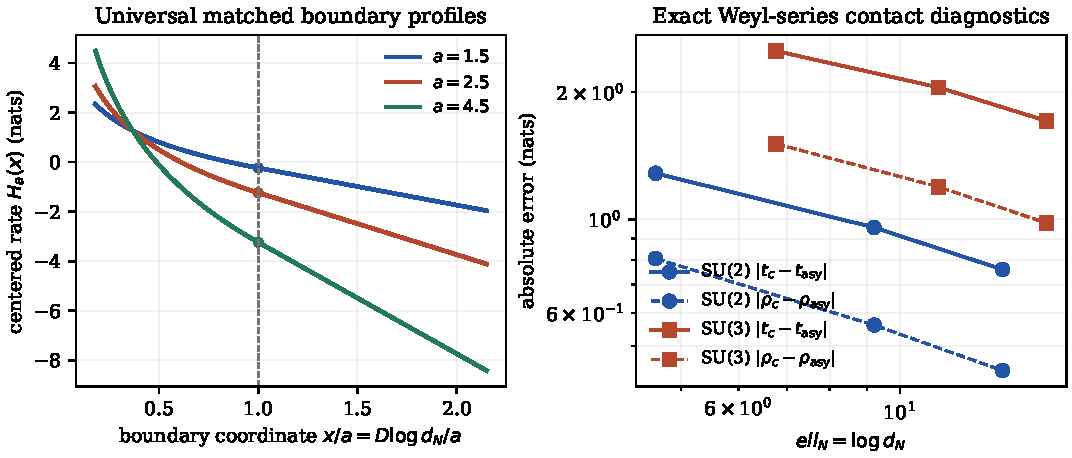
\includegraphics[width=\textwidth]{figures/semiclassical_universality.pdf}
 \caption{Left: the universal centered boundary profile
 $\mathcal H_a(x)$, with the horizontal coordinate normalized by its contact
 value $a$.  Dots mark the tangencies.  Right: bounded deterministic
 diagnostics from the exact Weyl series for symmetric powers of $SU(2)$ and
 $SU(3)$.  Slow convergence is expected because the theorem contains a
 $\log\log d_N$ correction.  Numerics illustrate the analytic theorem but
 are not used in its proof.}
 \label{fig:universality}
\end{figure}

\section{Examples}

\subsection{Symmetric powers of \texorpdfstring{$SU(q)$}{SU(q)}}

For $G=SU(q)$ and $\lambda=\omega_1$,
\[
 V_{N\omega_1}=\operatorname{Sym}^N(\C^q),
 \qquad d_N=\binom{N+q-1}{q-1},
 \qquad p=q-1,
 \qquad a=q-\frac12.
\]
Thus the macroscopic law is universal after division by
$\log\binom{N+q-1}{q-1}$, while the boundary contact occurs at
$D_c\log d_N\to q-1/2$.

For $SU(2)$, the scalar normalizer has the exact integral fixture
\[
 L_N(t)=\sum_{m\ge0}\frac{(t^2/4)^m}{(m!)^2(mN+1)}
 =\int_0^1 I_0(t x^{N/2})\,\dd x.                       \label{eq:SU2}
\]
This follows by inserting
$(mN+1)^{-1}=\int_0^1x^{mN}\dd x$ term by term.  It provides a transparent
one-dimensional check of every scale in the theorem.

For $SU(3)$,
\[
 d_{m,N}=\frac{(mN+1)(mN+2)}2,
 \qquad p=2,
 \qquad a=\frac52.
\]
The exact positive series remains inexpensive even for symbolic values of
$N$ spanning many orders of magnitude.

\subsection{Cartan powers of Slater-determinant orbits}

For $G=SU(n)$ and $\lambda=\omega_k$, the abstract projective coherent orbit
is $\operatorname{Gr}_{\C}(k,n)$ and
\[
 p=k(n-k),\qquad a=k(n-k)+\frac12.
\]
At $N=1$ the coherent vectors are unit Slater determinants in
$\Lambda^k\C^n$.  The ray $N\omega_k$ is the $N$th Cartan-power embedding of
the same projective orbit.  The present theorem applies to this embedding
sequence.  It should not be misread as an assertion that a single physical
fermionic Hilbert space has changed particle number without changing the
representation.

\section{Reproducibility and numerical scope}

The accompanying script evaluates \cref{eq:LN} by a positive recurrence,
computes $K_N'$ exactly from the normalized weights, and solves the global
contact equation
\[
 2K_N(t)-tK_N'(t)=0
\]
inside the analytically localized window.  It includes two exact Weyl
sequences:
\begin{center}
\begin{tabular}{@{}lll@{}}
\toprule
family & $d_{m,N}$ & $(p,a)$\\
\midrule
$SU(2)$ symmetric powers & $mN+1$ & $(1,3/2)$\\
$SU(3)$ symmetric powers & $(mN+1)(mN+2)/2$ & $(2,5/2)$\\
\bottomrule
\end{tabular}
\end{center}
The replay is deterministic, uses no Monte Carlo, and finishes in less than
one second on the reference machine.  The JSON output records the exact
contact residual, distortion, slope, asymptotic predictions, and convergence
errors.  \Cref{fig:universality} is generated from that frozen output and the
closed form \cref{eq:Ha}.  These checks diagnose constants and code paths;
they do not replace the proofs.

\section{Scope, novelty boundary, and open problems}

The theorem concerns a sequence of \emph{classical} random vectors supported
on phase-lifted coherent orbits.  Mutual information and rates are classical.
It is not quantum rate--distortion, a quantum channel-capacity theorem, a
click-only hidden-variable simulation, or a derivation of Born probabilities.

The following ingredients are prior machinery and are not claimed as new:
Weyl's dimension formula, Cartan components, integer-index coherent moment
extremality, Bessel asymptotics, entropy variational duality, and the exact
finite-$N$ RDF of \cite{Eriksson2026Coherent}.  The contribution is the
coupled highest-weight asymptotic theorem: its global contact localization,
dimension-universal constants, soft-activation expansion,
dimension-normalized exact-RDF limit, and matched boundary profile.

Three boundaries are important.
\begin{enumerate}[leftmargin=2em]
 \item Eventual uniqueness is proved for the global minimizing origin
 tangent only.  Other finite-$N$ stationary roots are not classified.
 \item The limit \cref{eq:macro} requires fixed $D>0$.  The boundary theorem
 handles $D\asymp1/\log d_N$, but exact zero distortion remains infinite.
 \item The abstract orbit is fixed while its Cartan embedding changes.
 Results for a fixed representation followed by $D\downarrow0$ are a
 different asymptotic problem.
\end{enumerate}

Natural next questions include third-order contact expansions retaining the
root-system-dependent $N^{-1}$ terms, moderate deviations between the soft
window and global contact, and extensions to sign-quotiented or projective
losses whose posterior-mean bodies differ from the phase-lifted orbitope.

\section{Conclusion}

Highest-weight scaling turns the exact coherent-orbit compression problem
into a universal phase diagram.  The normalizer first activates at
$\ell_N+a\log\ell_N+O(1)$, but the best time-sharing tangent waits until a
field twice as large to leading order.  The critical distortion shrinks as
$a/\ell_N$, the fixed-distortion RDF becomes the line $(1-D)\ell_N$, and a
matched $D\ell_N$ boundary layer retains the curved coherent branch and its
tangent in one explicit profile.  Writing the result in terms of the actual
Hilbert dimension removes every Weyl leading constant and leaves only half
the real source dimension.  The universality is therefore not an artifact of
one group or one orbit: it is the common semiclassical signature of the exact
Cartan-product rate--distortion mechanism.

\section*{Data and code availability}

The source package contains the LaTeX manuscript, bibliography, vector figure
and its generator, the bounded verification script, and frozen JSON output.
No external data set is used.  All floating-point values are diagnostic.

\section*{Use of AI tools}

AI tools assisted with literature discovery, algebraic replay, adversarial
checking, drafting, and layout inspection.  The named author takes
responsibility for the claims, proofs, citations, and release artifacts.  No
peer review or independent scientific validation is claimed.

\printbibliography

\end{document}
